\documentclass[14pt]{extbook}
\usepackage{multicol, enumerate, enumitem, hyperref, color, soul, setspace, parskip, fancyhdr} %General Packages
\usepackage{amssymb, amsthm, amsmath, latexsym, units, mathtools} %Math Packages
\everymath{\displaystyle} %All math in Display Style
% Packages with additional options
\usepackage[headsep=0.5cm,headheight=12pt, left=1 in,right= 1 in,top= 1 in,bottom= 1 in]{geometry}
\usepackage[usenames,dvipsnames]{xcolor}
\usepackage{dashrule}  % Package to use the command below to create lines between items
\newcommand{\litem}[1]{\item#1\hspace*{-1cm}\rule{\textwidth}{0.4pt}}
\pagestyle{fancy}
\lhead{Progress Quiz 8}
\chead{}
\rhead{Version B}
\lfoot{5493-4176}
\cfoot{}
\rfoot{Summer C 2021}
\begin{document}

\begin{enumerate}
\litem{
Choose the equation of the function graphed below.
\begin{center}
    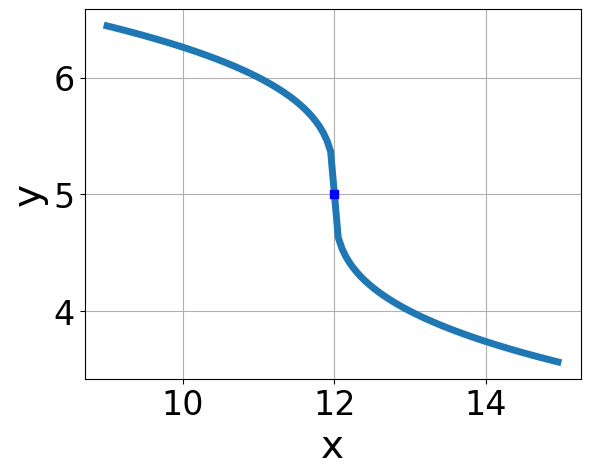
\includegraphics[width=0.5\textwidth]{../Figures/radicalGraphToEquationB.png}
\end{center}
\begin{enumerate}[label=\Alph*.]
\item \( f(x) = - \sqrt{x - 12} + 5 \)
\item \( f(x) = \sqrt{x - 12} + 5 \)
\item \( f(x) = - \sqrt{x + 12} + 5 \)
\item \( f(x) = \sqrt{x + 12} + 5 \)
\item \( \text{None of the above} \)

\end{enumerate} }
\litem{
Solve the radical equation below. Then, choose the interval(s) that the solution(s) belongs to.\[ \sqrt{-14 x^2 + 15} - \sqrt{-11 x} = 0 \]\begin{enumerate}[label=\Alph*.]
\item \( x \in [-0.94,-0.59] \)
\item \( x \in [1.22,2.18] \)
\item \( \text{All solutions lead to invalid or complex values in the equation.} \)
\item \( x_1 \in [-0.94, -0.59] \text{ and } x_2 \in [0.5,4.5] \)
\item \( x_1 \in [0.64, 0.89] \text{ and } x_2 \in [0.5,4.5] \)

\end{enumerate} }
\litem{
What is the domain of the function below?\[ f(x) = \sqrt[4]{-4 x + 6} \]\begin{enumerate}[label=\Alph*.]
\item \( [a, \infty), \text{where } a \in [1.04, 1.63] \)
\item \( (-\infty, a], \text{where } a \in [0.13, 0.89] \)
\item \( (-\infty, \infty) \)
\item \( (-\infty, a], \text{ where } a \in [1.08, 2.35] \)
\item \( [a, \infty), \text{where } a \in [-0.35, 1.23] \)

\end{enumerate} }
\litem{
Choose the graph of the equation below.\[ f(x) = \sqrt{x + 12} + 6 \]\begin{enumerate}[label=\Alph*.]
\begin{multicols}{2}\item 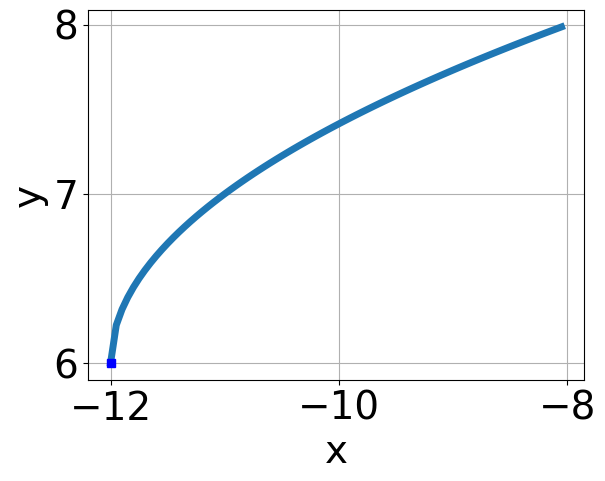
\includegraphics[width = 0.3\textwidth]{../Figures/radicalEquationToGraphCopyAB.png}\item 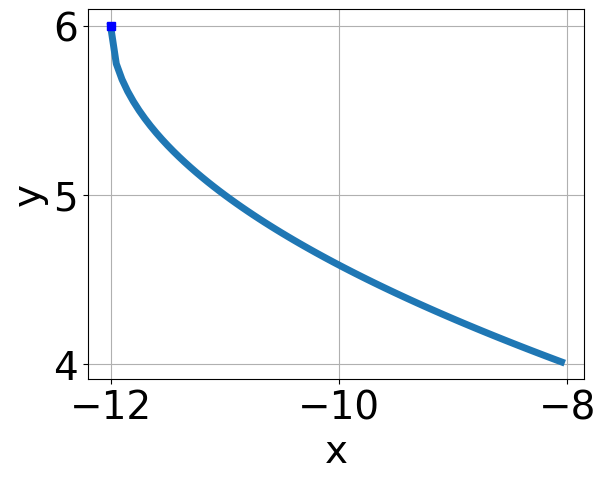
\includegraphics[width = 0.3\textwidth]{../Figures/radicalEquationToGraphCopyBB.png}\item 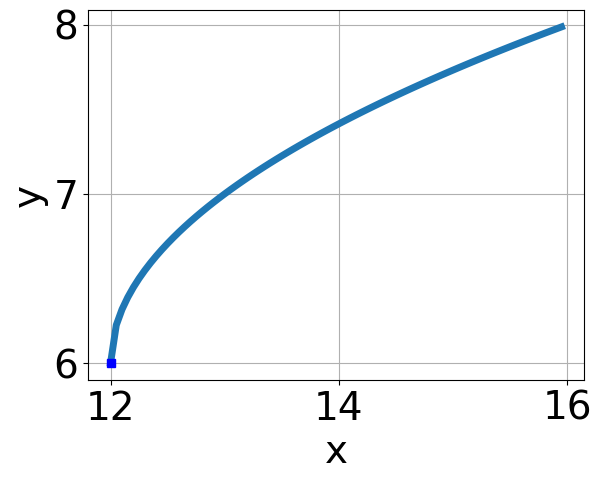
\includegraphics[width = 0.3\textwidth]{../Figures/radicalEquationToGraphCopyCB.png}\item 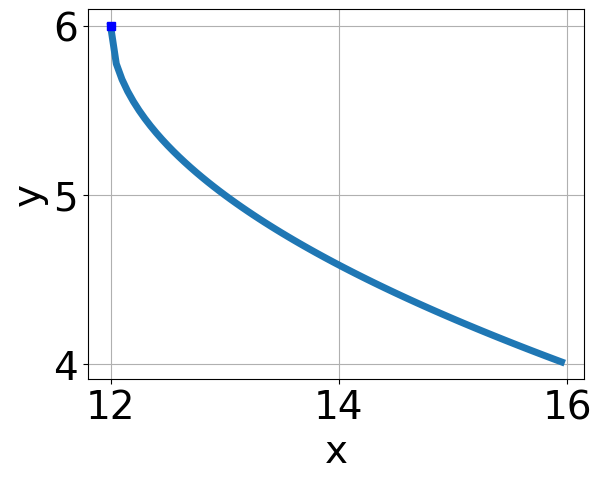
\includegraphics[width = 0.3\textwidth]{../Figures/radicalEquationToGraphCopyDB.png}\end{multicols}\item None of the above.
\end{enumerate} }
\litem{
Solve the radical equation below. Then, choose the interval(s) that the solution(s) belongs to.\[ \sqrt{-6 x - 4} - \sqrt{-8 x + 4} = 0 \]\begin{enumerate}[label=\Alph*.]
\item \( x_1 \in [-0.97, -0.43] \text{ and } x_2 \in [-0.5,1.5] \)
\item \( \text{All solutions lead to invalid or complex values in the equation.} \)
\item \( x \in [-0.5,0.24] \)
\item \( x_1 \in [-0.97, -0.43] \text{ and } x_2 \in [1,10] \)
\item \( x \in [2.34,4.82] \)

\end{enumerate} }
\litem{
Choose the equation of the function graphed below.
\begin{center}
    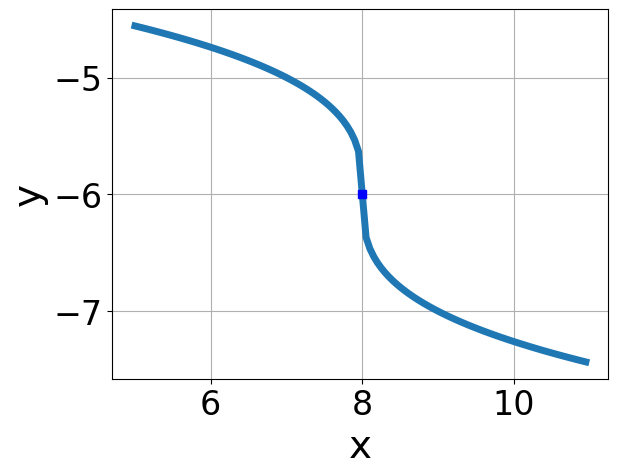
\includegraphics[width=0.5\textwidth]{../Figures/radicalGraphToEquationCopyB.png}
\end{center}
\begin{enumerate}[label=\Alph*.]
\item \( f(x) = \sqrt[3]{x - 8} - 6 \)
\item \( f(x) = \sqrt[3]{x + 8} - 6 \)
\item \( f(x) = - \sqrt[3]{x + 8} - 6 \)
\item \( f(x) = - \sqrt[3]{x - 8} - 6 \)
\item \( \text{None of the above} \)

\end{enumerate} }
\litem{
Solve the radical equation below. Then, choose the interval(s) that the solution(s) belongs to.\[ \sqrt{-9 x + 6} - \sqrt{-2 x + 8} = 0 \]\begin{enumerate}[label=\Alph*.]
\item \( \text{All solutions lead to invalid or complex values in the equation.} \)
\item \( x_1 \in [-1.48, -0.24] \text{ and } x_2 \in [-2.33,3.67] \)
\item \( x_1 \in [0.49, 1.27] \text{ and } x_2 \in [2,5] \)
\item \( x \in [-1.48,-0.24] \)
\item \( x \in [1.6,2.51] \)

\end{enumerate} }
\litem{
What is the domain of the function below?\[ f(x) = \sqrt[7]{7 x - 4} \]\begin{enumerate}[label=\Alph*.]
\item \( \text{The domain is } [a, \infty), \text{   where } a \in [-0.24, 1.15] \)
\item \( \text{The domain is } (-\infty, a], \text{   where } a \in [1.1, 2.2] \)
\item \( \text{The domain is } [a, \infty), \text{   where } a \in [0.88, 2.58] \)
\item \( (-\infty, \infty) \)
\item \( \text{The domain is } (-\infty, a], \text{   where } a \in [-0.2, 1.7] \)

\end{enumerate} }
\litem{
Choose the graph of the equation below.\[ f(x) = - \sqrt{x + 6} + 6 \]\begin{enumerate}[label=\Alph*.]
\begin{multicols}{2}\item 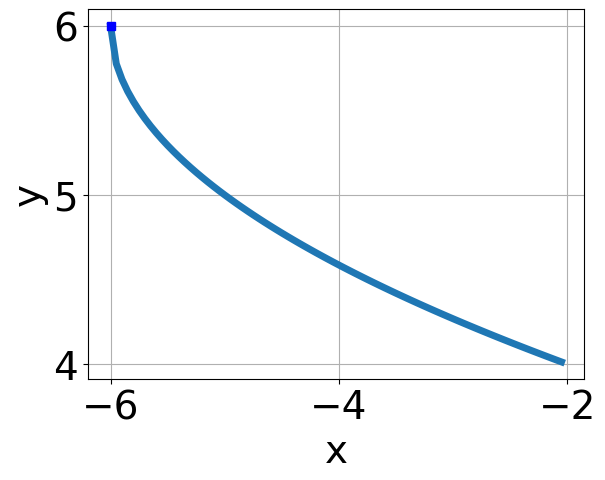
\includegraphics[width = 0.3\textwidth]{../Figures/radicalEquationToGraphAB.png}\item 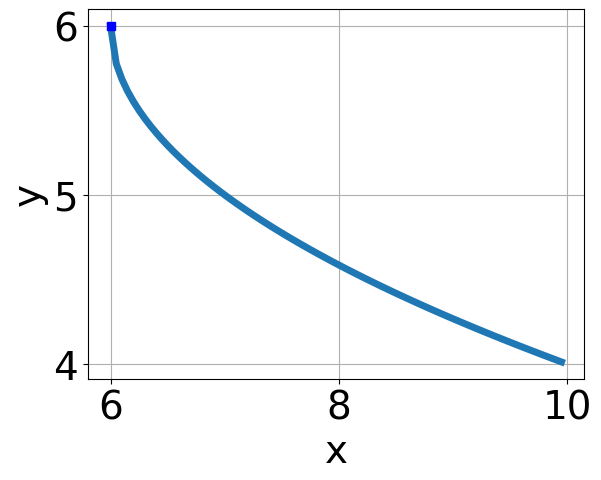
\includegraphics[width = 0.3\textwidth]{../Figures/radicalEquationToGraphBB.png}\item 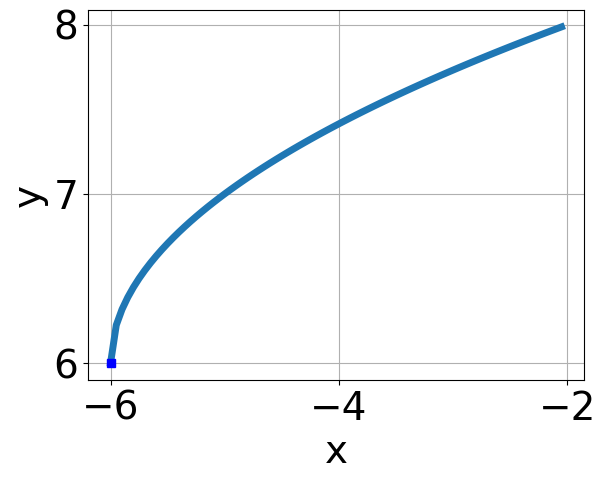
\includegraphics[width = 0.3\textwidth]{../Figures/radicalEquationToGraphCB.png}\item 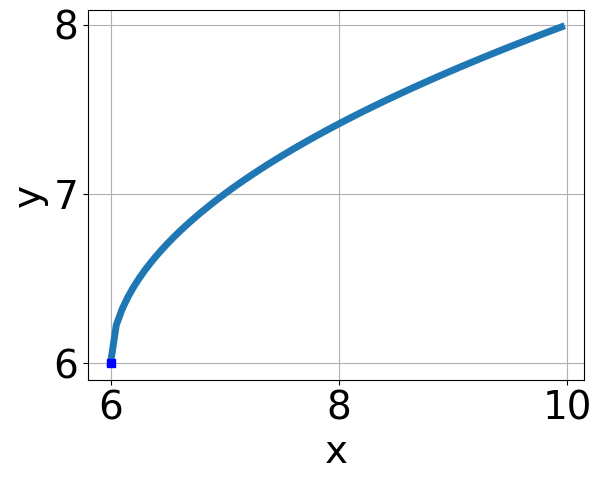
\includegraphics[width = 0.3\textwidth]{../Figures/radicalEquationToGraphDB.png}\end{multicols}\item None of the above.
\end{enumerate} }
\litem{
Solve the radical equation below. Then, choose the interval(s) that the solution(s) belongs to.\[ \sqrt{16 x^2 + 49} - \sqrt{-70 x} = 0 \]\begin{enumerate}[label=\Alph*.]
\item \( x_1 \in [-4.5, -2.6] \text{ and } x_2 \in [-2.88,1.12] \)
\item \( \text{All solutions lead to invalid or complex values in the equation.} \)
\item \( x \in [-4.5,-2.6] \)
\item \( x_1 \in [0, 4.5] \text{ and } x_2 \in [3.5,6.5] \)
\item \( x \in [-1.7,0.8] \)

\end{enumerate} }
\end{enumerate}

\end{document}